\section{Introduction.}  
In this work, we consider quantum circuits under the Clifford-free noise model. In this model, it is assumed that any of the Clifford gates, such as $S$, $H$, and $CZ$, can be applied perfectly. Additionally, the circuits have access to noisy magic states at an error rate of $p$, formulated as the mixed state $(1-p)\ket{T} + pZ\ket{T}$, where $p \in (0,1)$ is the probability that a given state is actually a faulty one and $\ket{T}= \frac{1}{\sqrt{2}}(\ket{0} + e^{i\frac{\pi}{4}}\ket{1})$ is a Magic State. Finally, the model allows for intermediate measurements and the application of Clifford gates controlled by the classical outcomes of the measurements. It has been shown that this model is quantum universal.

The Magic State Distillation Protocol is a quantum circuit in the Clifford-free noise model that consumes $n$ noisy magic states at an error rate of $p$ and outputs $k$ independent magic states at an error rate of $\varepsilon$. The previews constructions usually used self-\trig codes (\Cref{def:trig}) \cite{bravyi2012magic}, in which the logical $T^{k}$ gate can be computed transversally. Depending on how good the code is in terms of rate and distance, it can give a better gain in the reduction of the error rate and lower consumption of Magic states. This was shown in \ctt{cite it}. The standard approach of computing $T^{k}$ transversally gives a $\log^{\gamma}(\frac{1}{\varepsilon})$-overhead distillation protocol, where $\gamma = \log(\frac{n}{k}) / \log(d)$. \ctt{mention known $\gamma$ values and provide citations.}
For many years, the major focus was on giving a distillation protocol for which $\gamma \rightarrow 0$. Recently, \cite{constantoverheadmagicstatedistillation} succeeded in achieving this. This achievement raises the question of whether $\gamma = 0$ specifies the limit or if there exists a distillation protocol that consumes a sublinear amount of Magic states. We answer this question in the affirmative. Here, we show the existence and construction of protocols that consume $\sqrt{n}$ Magic States and produce, almost surely, $\Theta(n)$ perfect Magic States. We emphasize that the protocols output dependent states, i.e., if the protocol fails, then any of the $\Theta(n)$ outcomes is a faulty Magic state. This is why we put the phrase "Distillation" in quotation marks in the title.


\begin{theorem}[$\sqrt{n} \rightarrow n$ 'Distillation' (unformal)]
  There exists an efficient falut tolerance circuit, with respect to Clifford-free noise model, that with high probability produce asymptotically more Magic States than what it consumes.
\end{theorem}
\section{Notations, Definitions and Construction.} The notation used in this paper follows standard conventions for coding theory. We use $n$ to represent the length of the code, $k$ for the code's dimension, and $\rho$ for its rate. The minimum distance of the code will be denoted as $d$, and the relative distance, i.e., $d/n$, as $\delta$. In this paper, $n$ and $k$ will sometimes refer to the number of physical and logical bits. Codes will be denoted by a capital $C$ followed by either a subscript or superscript. When referring to multiple codes, we will use the above parameters as functions. For example, $\rho(C_{1})$ represents the rate of the code $C_{1}$. Square brackets are used to present all these parameters compactly, and we use them as follows: $C=[n,k,d]$ to declare a code with the specified length, dimension, and distance. Any theorem, lemma, or claim that states a statement that is true in the asymptotic sense refers to a family of codes. The parity check matrix of the code will be denoted as $H$, with the rows of $H$ representing the parity check equations. The generator matrix of the code will be denoted as $G$, with the rows of $G$ representing the basis of codewords. The syndrome of a received word will be denoted as $s$, which is the result of multiplying $r$ by the transpose of $H$. We use $C^\perp$ to denote the dual code of $C$, which is defined such that any codeword of it $z\in C^\perp$ is orthogonal to any $x\in C$, meaning $z\cdot x = 0$, where the product is defined as $x\cdot z = \sum_{i}{x_{i}z_{i}}$. $C^{\top}$ stands for the code obtained by taking the parity check matrix of $C$ and transposing it.

In this paper, we define the triple product $\mathbb{F}_2^{n}\times \mathbb{F}_2^{n}\times\mathbb{F}_2^{n} \rightarrow \mathbb{Z}$ as $|x\cdot y \cdot z| = \sum_{i}^{n}{x_{i}y_{i}z_{i}}$. Similarly, we define the binary product $|x \cdot y|$, noting that this product differs from the standard product by mapping into $\mathbb{Z}$ rather than $\mathbb{F}_{2}$. For $w \in \mathbb{F}_{2}^{n}$, we use the super operator $ \cdot |_{w} $ to map an operator originally defined in an $n$-dimensional space to an operator that only acts on coordinates restricted to $w$. For example, $x|_{w}$ is the vector in $\mathbb{F}_{2}^{|w|}$ obtained by taking the values of $x$ on coordinates where $w$ is not zero. $|x\cdot y|_{w} = \sum_{i:w_{i}\neq 0}{x_{i}y_{i}}$ and $C|_{w}$ is the code obtained by taking the codewords of $C$ restricted to $w$.

\begin{definition}
  \label{def:trig}
  Let $C$, $\tilde{C}$ be linear binary codes at the same length, We will say that $\tilde{C}$ is a \trig with respect to $C$ if: 
  \begin{enumerate}
    \item $\tilde{C} \subset C$
    \item $|x\cdot y \cdot z|$ is even for $x,y,z \in C$ such that at least one of $x,y,z$  belongs to $\tilde{C}$. 
    \item $|x\cdot y|$ is even for $x,y \in C$ such that at least one of $x,y$  belongs to $\tilde{C}$. 
  \end{enumerate}
  If a code $C$ is \trig with respect to itself then we will say that $C$ is a self \trig code. 
\end{definition}
For example, the empty code, that contains only the zero code word, i.e $C = \{ 0 \}$, is a \trig with respect to any code. In fact for proving \Cref{theorem:main} taking the empty code is sufficient. For other example, the \trig codes defined in \cite{bravyi2012magic} are \trig with respect to themself. 

A quantum code over $n$ qubits is an embedding of $\mathcal{H}_{2}^{\otimes k}$ as a subspace of $\mathcal{H}_{2}^{\otimes n}$. Similar to classical codes, we will call $n$ and $k$ the physical and logical qubits. The embeddings of states in $\mathcal{H}_{2}^{\otimes k}$ are called codewords or encoded states. In addition, we will use the term "logical operator" (i.e. logical $X_{i}$) to describe an operator that acts on the code space exactly as it would act on the logical space $\mathcal{H}_{2}^{\otimes k}$ (in our example, turning on and off the encoded state corresponds to the $i$th qubit exactly as $X_{i}$ acts as Pauli $X$ on the $i$th qubit in $\mathcal{H}_{2}^{\otimes k}$). We will denote by $X$ and $Z$ the single $X$ and $Z$ Pauli operators, by $X_{i}$ the application of $X$ on the $i$th qubit and nothing else (identity) on the rest of the qubits. By $X^{(v)}$ for some $v \in \mathbb{F}_{2}^{n}$, we mean the operator composed by applying $X$ on each of the qubits whose index is a non-trivial coordinate of $v$ and identity elsewhere. In a similar fashion, we define $Z^{(v)}$. When the context is clear, we will allow ourselves to omit the brackets, i.e. $Z^{v}$. The weight of a Pauli operator is the number of coordinates on which the operator acts non-trivially. Recall that the set of Pauli $+ I$ spans all the Hermitian matrices. We say that the Pauli weight of an operator is the maximal weight of a Pauli in its Pauli decomposition. For example, consider the operator $A = IXX + ZII$, the weight of $A$ is $2$. The distance of a quantum code is the minimal weight of an operator that takes one codeword to another. We use the standard bracket notation to describe quantum states and in addition, we define for a vector space $A \subset \mathbb{F}_{2}^{n}$ the notation $\ket{A}$ to represent the uniform superposition of all the vectors belonging to that space, namely: \begin{equation*}
  \begin{split}
\ket{A} = \frac{1}{\sqrt{|A|}}\sum_{x \in A}{\ket{x}}
  \end{split}
\end{equation*}
We define in the same way the notation to hold for affine spaces, $\ket{x +A}$. We will use $\propto$ to denote a quantum states up to normalization factor, for example $\ket{\psi} \propto \ket{0} + \ket{1}$ means that $\ket{\psi} = \frac{1}{\sqrt{2}}(\ket{0} + \ket{1})$.
A CSS code is a quantum code defined by a pair of classical codes $C_{X}$ and $C_{Z}$, satisfying $C_{Z}^{\perp} \subset C_{X}$, such that any codeword of it has the form $\ket{x + C_{Z}^\perp}$, where $x \in C_{X}$. We will use $Q$ to refer to a CSS code in general and use $\QQ$ to refer to the vectors associated with the $X$-generators or the encoded states in the computational basis. In the same way, $C_{Z}/C_{X}^{\perp}$ refers to the $Q$ in the phase basis. We will say that a CSS code $Q$ is a LDPC if $C_{X}$ and $C_{Z}$ are both LDPC codes. Our construction uses the classical Tanner code \cite{Tanner}, the expander codes \cite{ExpanderCodes}, and Hyperproduct product (quantum expanders) \cite{Leverrier_2015}, \cite{Tillich_2014}, \cite{overheadofquantumerrorcorrection}. We will not describe these constructions and refer the reader to those papers for further information.


\paragraph{}

%Comparing to previews construction, they usually used self \trig codes\cite{bravyi2012magic}, in which the logical $T^{k}$ can be computed transversally, then depend on how good the code are in terms of rate and distance, they give a better gain in the reduction of the error rate, in lower consumption amount of Magic states. It was shown \ctt{cite it}. That the standard approaching of computing $T^{k}$ transversally is giving a $\log^{\gamma}(\frac{1}{\varepsilon})$-overhead distillation protocol where $\gamma = \log(\frac{n}{k}) / \log(d)$. \ctt{mentions known $\gamma$ values and provide citations.}
%For many years the majority of the focus was about to give a distillation protocol for which $\gamma \rightarrow 0$, Recently \cite{constantoverheadmagicstatedistillation} succeed to achieve it. That achievement raise the question whether $\gamma =0$ specifying the limit, or if there exist distillation protocol that consume sublinear amount of Magic states. We answer on that question in affirmative. 

%The previews constructions usually used self-\trig codes \cite{bravyi2012magic}, in which the logical $T^{k}$ can be computed transversally. Depending on how good the code is in terms of rate and distance, it can give a better gain in the reduction of the error rate and lower consumption of Magic states. This was shown in \ctt{cite it}. The standard approach of computing $T^{k}$ transversally gives a $\log^{\gamma}(\frac{1}{\varepsilon})$-overhead distillation protocol, where $\gamma = \log(\frac{n}{k}) / \log(d)$. \ctt{mention known $\gamma$ values and provide citations.}
%For many years, the majority of the focus was on giving a distillation protocol for which $\gamma \rightarrow 0$. Recently, \cite{constantoverheadmagicstatedistillation} succeeded in achieving this. This achievement raises the question of whether $\gamma = 0$ specifies the limit or if there exists a distillation protocol that consumes a sublinear amount of Magic states. We answer this question in the affirmative.

\begin{theorem}[$\sqrt{n} \rightarrow n$ 'Distillation']
  \label{theorem:main}
There exists is $p_0 \in (0,1)$ such that for the Clifford-free noise model with an error rate $p < p_{0}$, there is a family of circuits that, for sufficiently large $n$, consume $\sqrt{n}$ noisy Magic States and with  probability greater than $1 - e^{-n^{1/8}}$ output $\Theta(n)$ perfect Magic States. Furthermore, both the width and depth of the circuits are linear in $n$.
\end{theorem}
Compared to the previous approaches, our construction does not use a self \trig code. Instead, we build a CSS code $Q$ for which there exists a subcode $\Mbas \subset \QQ$ with linear dimension, and non non-trivial distance, such that the restriction of $\Mbas$ to a vector $w \in C_{Z}/C_{X}^\perp$ is 'almost' \trig with respect to $(C_{X})|_{w}$. This condition 'almost' allows us to compute the logical $T^{\rho(\Mbas)n}$ by applying physical $T$ gates 'almost' only on the restricted bits. To overcome this 'almost' issue, we show that by choosing the code $Q$ to be an LDPC code, and such that there exists a vector $w\in C_{Z}/C_{X}^\perp$ with weight $|w| = \Theta(n^\frac{1}{4})$, Then the number of $T$ gates that need to be applied in a non-transversal fashion is sublinear. We then apply one of the previous distillation protocols to ensure that we have fresh magic states, which can effectively be thought of as perfect, to compute the non-transversal $T$ gates.

\subsection{The Protocol's Description.} 
We are about to describe the circuit. \Cref{def:thecode} defines a quantum code $Q$, in which the main computation occurs. \Cref{def:subcode} defines a subspace $\Mbas \subset \QQ$ and a $Z$-generator $w$ such $\Mbas|_{w}$ is \trig with respect to $(C_{X})|_{w}$. Lastly, \Cref{def:gates} defines the quantum gates $\mathcal{C}$, $\mathcal{E}$ and $\mathcal{D}$ stand for low-$T$ gate, encoder and decoder respectively, In \Cref{fig:circ} an hypotactic valid scheme of main routine is shown, for capture the full figure it's left to chain the drawn circuit constant number of time.  
\begin{definition}
  \label{def:thecode}
Let $\Delta$ be a constant integer, $C_{0}$ and $\tilde{C}_{0}$ be codes over $\Delta$ bits such that $\tilde{C}_{0}$ is \trig with respect to $C^{\perp}_{0}$. $C_{0}$ has parameters $\Delta[1,\delta_{0},\rho_{0}]$, and $C_{0}^\top$ has relative distance greater than $\delta_{0}$. Let $\Ctan$ be a Tanner code, defined by taking an expander graph with good expansion and $C_{0}$ as the small code. Let $\Cin$ be the dual-tensor code obtained by taking $(\Ctan^\perp \otimes \Ctan^\perp )^\perp$. Note that first, this code has a positive rate and $\Theta(\sqrt{n})$ distance. Second, this code is an LDPC code as well. Also, notice that $\Cin^{\top}$ is obtained by transporting the parity check matrix, and therefore equals to $(\Ctan^{\top, \perp} \otimes \Ctan^{\top, \perp} )^\perp$. Hence, $\Cin^{\top}$ has a square root distance as well.

Let $Q$ be the CSS code obtained by taking the \Hyp of $\Cin$ with itself. So, $Q$ is a quantum qLDPC code with parameters $[n, \Theta(n^{\frac{1}{4}}), \Theta(n)]$. The notations $Q,\Ctan, \Cin, \tilde{C}_{0}, C_{0}$ will keep these definitions for the rest of the paper.
\end{definition}
For further explanation on dual-tensor, please refer to \cite{leverrier2022quantum}, \cite{Dinur}, and \cite{Pavel}. We rely on the main theorem in \cite{Tillich_2014} for the \Hyp code distance and rate.

The main advantage of using the dual-tensor and \Hyp is that their bases can be easily understood in terms of the codes being multiplied to obtain them. For the dual-tensor $(C^{\perp}\otimes C^{\perp})^{\perp} = C\otimes \mathbb{F}_{2}^{n} \oplus \mathbb{F}_{2}^{n} \otimes C$, one can think of the codewords as $n\times n$ binary matrices and take the collection of imposing single generators of $C$ on the rows or columns as the code base. In the \Hyp, the code words can be thought of as assignments of bits on two matrices: the first at size $n(C) \times n(C)$, while the second is at size $n(C^\top) \times n(C^\top)$. Any generator of $C_{X}$ either imposes a $C$ generator on one of the rows of the first matrix or imposes a $C^{\top}$ generator on one of the columns of the second matrix. In our case, we can imagine that both the $X$ and $Z$ generators of $Q$ correspond to setting a generator of $\Ctan$, $\Ctan^\top$ on a 'row' of the 4D cube.


\begin{definition}
  \label{def:subcode}  
Consider the code $Q$, defined in \cref{def:thecode} in the computation base $\QQ$. Let $x_{0}$ be a codeword of $\QQ$. Denote by $w \in \mathbb{F}_{2}^{n}$ the binary string that represents the $Z$-generator that anti-commutes with the $X$-generator corresponding to $x_{0}$. Let $\mathcal{X} = \{x_{0}, x_{1}, .. x_{k^\prime}\} \in \mathbb{F}_{2}^{n}$ be a subset of a basis for the code $\QQ$. Such $\left(\text{span } \mathcal{X}/x_0 \ \right)|_{w}$ is a \trig code with respect to $C_{X}|_{w}$. Let us denote by $\Mbas$ the basis $\{ y_{1}, y_{2}, .., y_{k^\prime} \} \in \mathbb{F}_{2}^{n}$ defined as follows: $ y_{i} = x_{j} + x_{0}$.
\end{definition}

 \Cref{claim:notempty} states that $\Mbas$ is not empty and even has linear size at $n$.


 \begin{definition}
   \label{def:gates} 
 Denote by $E$ the circuit that encodes the $i$th logical bit into $\ket{y_{i}+C_{Z}^{\perp}}$, By $T^{(w)}$ the application of $T$ gates on the qubits for which $w$ acts non-trivially, meaning $T^{(w)}$ is a tensor product of $T$'s and $I$'s where on the $i$th qubit $T^{(w)}$ applies $T$ if $w_{i}$ equals $1$, and identity otherwise. By $D$ denote the gate that decodes binary strings in $\mathbb{F}_{2}^{n}$ back into the logical space, $D$ is also responsible to correct errors.
 Finally, denote by $\mathcal{C}$ a non Clifford gate, which contains at most $o(n^{\frac{1}{4}})$ Magic States, and by $\mathcal{D}$ an $n^{2}$-overhead  Magic Distillation Protocol, that consume $\Theta(\sqrt{n})$ magic and produce $O(n^\frac{1}{4})$ Magic States, with error rate less than $2^{-\alpha n}$.     
 \end{definition}

\begin{figure}
  \label{fig:circ}
  \noindent %\includegraphics{example-image-c} 
  \scalebox{1.7}{ 
  %! \usetikzlibrary{decorations.pathreplacing,decorations.pathmorphing}
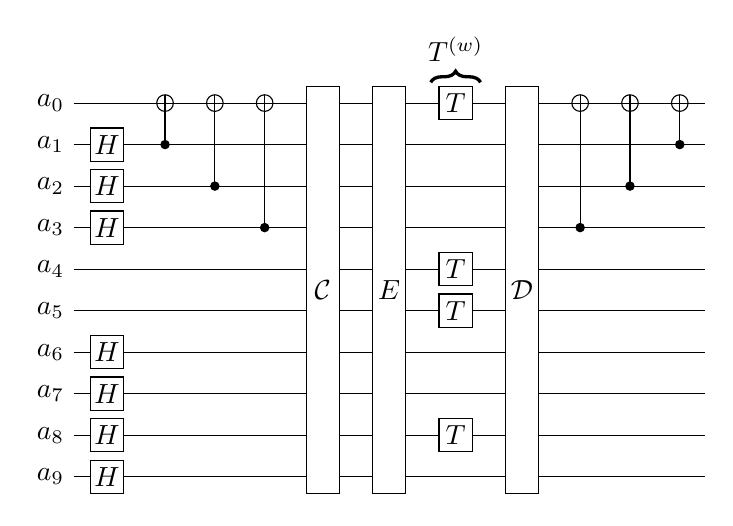
\begin{tikzpicture}[scale=1.000000,x=1pt,y=1pt]
\filldraw[color=white] (0.000000, -7.500000) rectangle (228.000000, 142.500000);
% Drawing wires
% Line 1: a0 W a_0
\draw[color=black] (0.000000,135.000000) -- (228.000000,135.000000);
\draw[color=black] (0.000000,135.000000) node[left] {$a_0$};
% Line 2: a1 W a_1
\draw[color=black] (0.000000,120.000000) -- (228.000000,120.000000);
\draw[color=black] (0.000000,120.000000) node[left] {$a_1$};
% Line 3: a2 W a_2
\draw[color=black] (0.000000,105.000000) -- (228.000000,105.000000);
\draw[color=black] (0.000000,105.000000) node[left] {$a_2$};
% Line 4: a3 W a_3
\draw[color=black] (0.000000,90.000000) -- (228.000000,90.000000);
\draw[color=black] (0.000000,90.000000) node[left] {$a_3$};
% Line 5: a4 W a_4
\draw[color=black] (0.000000,75.000000) -- (228.000000,75.000000);
\draw[color=black] (0.000000,75.000000) node[left] {$a_4$};
% Line 6: a5 W a_5
\draw[color=black] (0.000000,60.000000) -- (228.000000,60.000000);
\draw[color=black] (0.000000,60.000000) node[left] {$a_5$};
% Line 7: a6 W a_6
\draw[color=black] (0.000000,45.000000) -- (228.000000,45.000000);
\draw[color=black] (0.000000,45.000000) node[left] {$a_6$};
% Line 8: a7 W a_7
\draw[color=black] (0.000000,30.000000) -- (228.000000,30.000000);
\draw[color=black] (0.000000,30.000000) node[left] {$a_7$};
% Line 9: a8 W a_8
\draw[color=black] (0.000000,15.000000) -- (228.000000,15.000000);
\draw[color=black] (0.000000,15.000000) node[left] {$a_8$};
% Line 10: a9 W a_9
\draw[color=black] (0.000000,0.000000) -- (228.000000,0.000000);
\draw[color=black] (0.000000,0.000000) node[left] {$a_9$};
% Done with wires; drawing gates
% Line 13: a1 G $H$
\begin{scope}
\draw[fill=white] (12.000000, 120.000000) +(-45.000000:8.485281pt and 8.485281pt) -- +(45.000000:8.485281pt and 8.485281pt) -- +(135.000000:8.485281pt and 8.485281pt) -- +(225.000000:8.485281pt and 8.485281pt) -- cycle;
\clip (12.000000, 120.000000) +(-45.000000:8.485281pt and 8.485281pt) -- +(45.000000:8.485281pt and 8.485281pt) -- +(135.000000:8.485281pt and 8.485281pt) -- +(225.000000:8.485281pt and 8.485281pt) -- cycle;
\draw (12.000000, 120.000000) node {$H$};
\end{scope}
% Line 14: a2 G $H$
\begin{scope}
\draw[fill=white] (12.000000, 105.000000) +(-45.000000:8.485281pt and 8.485281pt) -- +(45.000000:8.485281pt and 8.485281pt) -- +(135.000000:8.485281pt and 8.485281pt) -- +(225.000000:8.485281pt and 8.485281pt) -- cycle;
\clip (12.000000, 105.000000) +(-45.000000:8.485281pt and 8.485281pt) -- +(45.000000:8.485281pt and 8.485281pt) -- +(135.000000:8.485281pt and 8.485281pt) -- +(225.000000:8.485281pt and 8.485281pt) -- cycle;
\draw (12.000000, 105.000000) node {$H$};
\end{scope}
% Line 15: a3 G $H$
\begin{scope}
\draw[fill=white] (12.000000, 90.000000) +(-45.000000:8.485281pt and 8.485281pt) -- +(45.000000:8.485281pt and 8.485281pt) -- +(135.000000:8.485281pt and 8.485281pt) -- +(225.000000:8.485281pt and 8.485281pt) -- cycle;
\clip (12.000000, 90.000000) +(-45.000000:8.485281pt and 8.485281pt) -- +(45.000000:8.485281pt and 8.485281pt) -- +(135.000000:8.485281pt and 8.485281pt) -- +(225.000000:8.485281pt and 8.485281pt) -- cycle;
\draw (12.000000, 90.000000) node {$H$};
\end{scope}
% Line 16: a6 G $H$
\begin{scope}
\draw[fill=white] (12.000000, 45.000000) +(-45.000000:8.485281pt and 8.485281pt) -- +(45.000000:8.485281pt and 8.485281pt) -- +(135.000000:8.485281pt and 8.485281pt) -- +(225.000000:8.485281pt and 8.485281pt) -- cycle;
\clip (12.000000, 45.000000) +(-45.000000:8.485281pt and 8.485281pt) -- +(45.000000:8.485281pt and 8.485281pt) -- +(135.000000:8.485281pt and 8.485281pt) -- +(225.000000:8.485281pt and 8.485281pt) -- cycle;
\draw (12.000000, 45.000000) node {$H$};
\end{scope}
% Line 17: a7 G $H$
\begin{scope}
\draw[fill=white] (12.000000, 30.000000) +(-45.000000:8.485281pt and 8.485281pt) -- +(45.000000:8.485281pt and 8.485281pt) -- +(135.000000:8.485281pt and 8.485281pt) -- +(225.000000:8.485281pt and 8.485281pt) -- cycle;
\clip (12.000000, 30.000000) +(-45.000000:8.485281pt and 8.485281pt) -- +(45.000000:8.485281pt and 8.485281pt) -- +(135.000000:8.485281pt and 8.485281pt) -- +(225.000000:8.485281pt and 8.485281pt) -- cycle;
\draw (12.000000, 30.000000) node {$H$};
\end{scope}
% Line 18: a8 G $H$
\begin{scope}
\draw[fill=white] (12.000000, 15.000000) +(-45.000000:8.485281pt and 8.485281pt) -- +(45.000000:8.485281pt and 8.485281pt) -- +(135.000000:8.485281pt and 8.485281pt) -- +(225.000000:8.485281pt and 8.485281pt) -- cycle;
\clip (12.000000, 15.000000) +(-45.000000:8.485281pt and 8.485281pt) -- +(45.000000:8.485281pt and 8.485281pt) -- +(135.000000:8.485281pt and 8.485281pt) -- +(225.000000:8.485281pt and 8.485281pt) -- cycle;
\draw (12.000000, 15.000000) node {$H$};
\end{scope}
% Line 19: a9 G $H$
\begin{scope}
\draw[fill=white] (12.000000, -0.000000) +(-45.000000:8.485281pt and 8.485281pt) -- +(45.000000:8.485281pt and 8.485281pt) -- +(135.000000:8.485281pt and 8.485281pt) -- +(225.000000:8.485281pt and 8.485281pt) -- cycle;
\clip (12.000000, -0.000000) +(-45.000000:8.485281pt and 8.485281pt) -- +(45.000000:8.485281pt and 8.485281pt) -- +(135.000000:8.485281pt and 8.485281pt) -- +(225.000000:8.485281pt and 8.485281pt) -- cycle;
\draw (12.000000, -0.000000) node {$H$};
\end{scope}
% Line 23: +a0 a1
\draw (33.000000,135.000000) -- (33.000000,120.000000);
\begin{scope}
\draw[fill=white] (33.000000, 135.000000) circle(3.000000pt);
\clip (33.000000, 135.000000) circle(3.000000pt);
\draw (30.000000, 135.000000) -- (36.000000, 135.000000);
\draw (33.000000, 132.000000) -- (33.000000, 138.000000);
\end{scope}
\filldraw (33.000000, 120.000000) circle(1.500000pt);
% Line 24: +a0 a2
\draw (51.000000,135.000000) -- (51.000000,105.000000);
\begin{scope}
\draw[fill=white] (51.000000, 135.000000) circle(3.000000pt);
\clip (51.000000, 135.000000) circle(3.000000pt);
\draw (48.000000, 135.000000) -- (54.000000, 135.000000);
\draw (51.000000, 132.000000) -- (51.000000, 138.000000);
\end{scope}
\filldraw (51.000000, 105.000000) circle(1.500000pt);
% Line 25: +a0 a3
\draw (69.000000,135.000000) -- (69.000000,90.000000);
\begin{scope}
\draw[fill=white] (69.000000, 135.000000) circle(3.000000pt);
\clip (69.000000, 135.000000) circle(3.000000pt);
\draw (66.000000, 135.000000) -- (72.000000, 135.000000);
\draw (69.000000, 132.000000) -- (69.000000, 138.000000);
\end{scope}
\filldraw (69.000000, 90.000000) circle(1.500000pt);
% Line 28: a0 a1 a2 a3 a4 a5 a6 a7 a8 a9 G $ \mathcal{C}$
\draw (90.000000,135.000000) -- (90.000000,0.000000);
\begin{scope}
\draw[fill=white] (90.000000, 67.500000) +(-45.000000:8.485281pt and 103.944697pt) -- +(45.000000:8.485281pt and 103.944697pt) -- +(135.000000:8.485281pt and 103.944697pt) -- +(225.000000:8.485281pt and 103.944697pt) -- cycle;
\clip (90.000000, 67.500000) +(-45.000000:8.485281pt and 103.944697pt) -- +(45.000000:8.485281pt and 103.944697pt) -- +(135.000000:8.485281pt and 103.944697pt) -- +(225.000000:8.485281pt and 103.944697pt) -- cycle;
\draw (90.000000, 67.500000) node {$ \mathcal{C}$};
\end{scope}
% Line 29: a0 a1 a2 a3 a4 a5 a6 a7 a8 a9 G $ E $
\draw (114.000000,135.000000) -- (114.000000,0.000000);
\begin{scope}
\draw[fill=white] (114.000000, 67.500000) +(-45.000000:8.485281pt and 103.944697pt) -- +(45.000000:8.485281pt and 103.944697pt) -- +(135.000000:8.485281pt and 103.944697pt) -- +(225.000000:8.485281pt and 103.944697pt) -- cycle;
\clip (114.000000, 67.500000) +(-45.000000:8.485281pt and 103.944697pt) -- +(45.000000:8.485281pt and 103.944697pt) -- +(135.000000:8.485281pt and 103.944697pt) -- +(225.000000:8.485281pt and 103.944697pt) -- cycle;
\draw (114.000000, 67.500000) node {$ E $};
\end{scope}
% Line 32: a0 G $T$
\begin{scope}
\draw[fill=white] (138.000000, 135.000000) +(-45.000000:8.485281pt and 8.485281pt) -- +(45.000000:8.485281pt and 8.485281pt) -- +(135.000000:8.485281pt and 8.485281pt) -- +(225.000000:8.485281pt and 8.485281pt) -- cycle;
\clip (138.000000, 135.000000) +(-45.000000:8.485281pt and 8.485281pt) -- +(45.000000:8.485281pt and 8.485281pt) -- +(135.000000:8.485281pt and 8.485281pt) -- +(225.000000:8.485281pt and 8.485281pt) -- cycle;
\draw (138.000000, 135.000000) node {$T$};
\end{scope}
% Line 33: a4 G $T$
\begin{scope}
\draw[fill=white] (138.000000, 75.000000) +(-45.000000:8.485281pt and 8.485281pt) -- +(45.000000:8.485281pt and 8.485281pt) -- +(135.000000:8.485281pt and 8.485281pt) -- +(225.000000:8.485281pt and 8.485281pt) -- cycle;
\clip (138.000000, 75.000000) +(-45.000000:8.485281pt and 8.485281pt) -- +(45.000000:8.485281pt and 8.485281pt) -- +(135.000000:8.485281pt and 8.485281pt) -- +(225.000000:8.485281pt and 8.485281pt) -- cycle;
\draw (138.000000, 75.000000) node {$T$};
\end{scope}
% Line 34: a5 G $T$
\begin{scope}
\draw[fill=white] (138.000000, 60.000000) +(-45.000000:8.485281pt and 8.485281pt) -- +(45.000000:8.485281pt and 8.485281pt) -- +(135.000000:8.485281pt and 8.485281pt) -- +(225.000000:8.485281pt and 8.485281pt) -- cycle;
\clip (138.000000, 60.000000) +(-45.000000:8.485281pt and 8.485281pt) -- +(45.000000:8.485281pt and 8.485281pt) -- +(135.000000:8.485281pt and 8.485281pt) -- +(225.000000:8.485281pt and 8.485281pt) -- cycle;
\draw (138.000000, 60.000000) node {$T$};
\end{scope}
% Line 35: a8 G $T$
\begin{scope}
\draw[fill=white] (138.000000, 15.000000) +(-45.000000:8.485281pt and 8.485281pt) -- +(45.000000:8.485281pt and 8.485281pt) -- +(135.000000:8.485281pt and 8.485281pt) -- +(225.000000:8.485281pt and 8.485281pt) -- cycle;
\clip (138.000000, 15.000000) +(-45.000000:8.485281pt and 8.485281pt) -- +(45.000000:8.485281pt and 8.485281pt) -- +(135.000000:8.485281pt and 8.485281pt) -- +(225.000000:8.485281pt and 8.485281pt) -- cycle;
\draw (138.000000, 15.000000) node {$T$};
\end{scope}
% Line 40: a0 a1 a2 a3 a4 a5 a6 a7 a8 a9 G $ \mathcal{D}$
\draw (162.000000,135.000000) -- (162.000000,0.000000);
\begin{scope}
\draw[fill=white] (162.000000, 67.500000) +(-45.000000:8.485281pt and 103.944697pt) -- +(45.000000:8.485281pt and 103.944697pt) -- +(135.000000:8.485281pt and 103.944697pt) -- +(225.000000:8.485281pt and 103.944697pt) -- cycle;
\clip (162.000000, 67.500000) +(-45.000000:8.485281pt and 103.944697pt) -- +(45.000000:8.485281pt and 103.944697pt) -- +(135.000000:8.485281pt and 103.944697pt) -- +(225.000000:8.485281pt and 103.944697pt) -- cycle;
\draw (162.000000, 67.500000) node {$ \mathcal{D}$};
\end{scope}
% Line 42: +a0 a3
\draw (183.000000,135.000000) -- (183.000000,90.000000);
\begin{scope}
\draw[fill=white] (183.000000, 135.000000) circle(3.000000pt);
\clip (183.000000, 135.000000) circle(3.000000pt);
\draw (180.000000, 135.000000) -- (186.000000, 135.000000);
\draw (183.000000, 132.000000) -- (183.000000, 138.000000);
\end{scope}
\filldraw (183.000000, 90.000000) circle(1.500000pt);
% Line 43: +a0 a2
\draw (201.000000,135.000000) -- (201.000000,105.000000);
\begin{scope}
\draw[fill=white] (201.000000, 135.000000) circle(3.000000pt);
\clip (201.000000, 135.000000) circle(3.000000pt);
\draw (198.000000, 135.000000) -- (204.000000, 135.000000);
\draw (201.000000, 132.000000) -- (201.000000, 138.000000);
\end{scope}
\filldraw (201.000000, 105.000000) circle(1.500000pt);
% Line 44: +a0 a1
\draw (219.000000,135.000000) -- (219.000000,120.000000);
\begin{scope}
\draw[fill=white] (219.000000, 135.000000) circle(3.000000pt);
\clip (219.000000, 135.000000) circle(3.000000pt);
\draw (216.000000, 135.000000) -- (222.000000, 135.000000);
\draw (219.000000, 132.000000) -- (219.000000, 138.000000);
\end{scope}
\filldraw (219.000000, 120.000000) circle(1.500000pt);
% Done with gates; drawing ending labels
% Done with ending labels; drawing cut lines and comments
% Line 38: @ 6 6 % $T^{(w)}$
\draw[decorate,decoration={brace,amplitude = 4.000000pt},very thick] (129.000000,142.500000) -- (147.000000,142.500000);
\draw (138.000000, 146.500000) node[text width=144pt,above,text centered] {$T^{(w)}$};
% Done with comments
\end{tikzpicture}

}
\caption{ The circuit.   }
\end{figure}

